\section{Zielsetzung}
\label{sec:Zielsetzung}
Das Ziel des Versuchs ist es, die Schwingungsdauer und Schwebungsdauer bei gekoppelten Pendeln in verschiedenen Schwingungsarten zu bestimmen.

\section{Theorie}
\label{sec:Theorie}

\subsection{Das Fadenpendel} % (fold)
\label{sub:Fadenpendel}
Das Fadenpendel besteht aus einer Masse $m$ und einem Faden der Länge $l$, wobei dieser idealerweise keine Masse besitzt.
Es wirkt die Gewichtskraft $F=m\,a$ als rücktreibende Kraft bei der Auslenkung des Pendels aus seiner Ruhelage.
Dadurch entsteht ein Drehmoment $M=D_p\, \phi$ auf das Pendel, wobei $\phi$ der Auslenkwinkel und $D_p$ die Winkelrichtung des Pendels ist.
Für kleine Auslenkungen gilt die Kleinwinkelnäherung und sodass die Bewegungsgleichung
\begin{equation}
    J \, \ddot{\phi} + D_p \, \phi = 0
\end{equation}
mit $J$ als Trägheitsmoment.
Die Lösung der Gleichung beschreibt eine harmonsische Schwingung mit der Schwingungsfrequenz
\begin{equation}
    \omega = \sqrt{\frac{D_p}{J}} = \sqrt{\frac{g}{l}}
\end{equation}
Bei kleinen Auslenkungen ist die Schwingungsdauer außerdem unabhängig von den Pendelmassen und dem Auslenkwinkel.
 
% subsection Fadenpendel (end)

\subsection{Gekoppelte Schwingungen} % (fold)
\label{subsec:Schwingungen}
 Bei einer Kopplung zweier identischen Pendel durch eine Feder wirkt ein weiteres Drehmoment auf jedes Pendel.
 Dadurch dass die Pendel jetzt über eine Feder gekoppelt schwingen sie nicht mehr unabhängig voneinander und es gilt das Hookesches Gesetz
 \begin{equation*}
     F(x) = -k \, x ,
 \end{equation*}
 wobei $k$ die Federkonstante und $x$ die Auslenkung ist.
 Die Bewegungsgleichung wird zu einem System gekoppelter Differentialgleichungen
 \begin{align}
     J \, \ddot{\phi_1} + D \phi_1 &= D_F (\phi_2 - \phi_1) \\
     J \, \ddot{\phi_2} + D \phi_2 &= D_F (\phi_1 - \phi_2)
 \end{align}
 umformt, wobei die linke Seite der Gleichung die Schwingung des einzelnen Pendels ist und die rechte Seite die Kopplung betrachtet.
 Die Schwingungsgleichung kann entkoppelt werden bei der richtigen Wahl der Winkel und können so als eine Überlagerung zweier Eigenschwingungen dargestellt werden.
 Die Schwingungsarten sind abhängig von den Anfangsbedingungen $\phi(0)$ und $\dot{\phi(0)}$. 

\subsubsection{Gleichsinnige Schwingungen}
\label{subsec:Gleich}
\begin{minipage}[t]{0.5\textwidth}
Die zwei identischen Pendel werden um den gleichen Winkel $\phi_1 = \phi_2$ ausgelenkt, sodass die Kopplungsfeder keine Kraft auf die Pendel ausübt.
Die rücktreibende Kraft wird nur von der Gravitation verursacht.
Mit der Schwingungsfrequenz der gleichsinnigen Schwingung
\begin{equation}
    \omega_+ = \sqrt{\frac{g}{l}}
    \label{eqn:omega+}
\end{equation}
ergibt sich die Schwingungsdauer zu
\begin{equation}
    T_+ = 2 \pi \sqrt{\frac{l}{g}}
    \label{eqn:T+}
\end{equation}
\end{minipage}
\begin{minipage}[t]{0.5\textwidth}
    \begin{figure}[H]
        \centering
        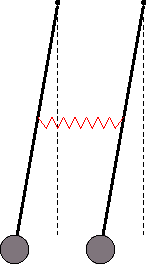
\includegraphics[width=0.45\textwidth]{build/Abb_1.pdf}
\caption{\\Abbild der gleichsinnigen Schwingung. \cite{V106}}
        \label{fig:gleich}
      \end{figure}
\end{minipage}
\subsubsection{Gegenseitige Schwingung}

\begin{minipage}[t]{0.5\textwidth}
\label{subsec:Gegen}
Die zwei identischen Pendel werden um den entgegengesetzten Winkel $\phi_1 = \phi_2$ ausgelenkt.
In diesem fall übt die Kopplungsfeder eine gleich große und entgegengesetzten Kraft auf die einzelnen Pendel aus.
Mit der Schwingungsfrequenz
\begin{equation}
    \omega_- = \sqrt{\frac{g}{l} + \frac{2K}{l}}
    \label{eqn:omega-}
\end{equation}
der symmetrischen Schwingung ergibt sich die Schwingungsdauer
\begin{equation}
    T_- = 2\pi \sqrt{\frac{l}{g+2K}}.
    \label{eqn:T-}
\end{equation}
Wobei die Kopplungskonstante der Feder durch das K dargestellt wird.
\end{minipage}
\begin{minipage}[t]{0.5\textwidth}
    \begin{figure}[H]
        \centering
        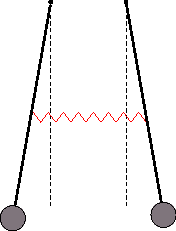
\includegraphics[width=0.5\textwidth]{build/Abb_2.pdf}
        \caption{Abbild der \\gegensinnigen Schwingung. \cite{V106}}
        \label{fig:gegen}
      \end{figure}
\end{minipage}
\subsubsection{Gekoppelte Schwingungen}
\label{subsec:Gekoppelt}
\begin{minipage}[t]{0.5\textwidth}
In diesem Fall ist bleibt eines der Pendel in Ruhelage $\phi_1=0$ und das andere idealistische Pendel wird um den Winkel $\phi_2 \neq 0$ ausgelenkt.
Beim Schwingen überträgt das erste Pendel seine Energie auf das zweite, sodass das zweite langsam anfängt zu schwingen.
Das zweite Pendel überträgt seine Energie wieder auf das Erste, welches anfängt zu schwingen.
Die Amplituden sind wie eine Glockenkurve. 
Ihr Maximum erreichen sie, wenn das andere Pendel zur Ruhe kommt.
Diese vollständige Energieübertragung wiederholt sich immer wieder und die Zeit zwischen den zwei Stillständen wird Schwebungsdauer 
\begin{equation}
    T_S=\frac{T+\,T_-}{T_+-T_-}
    \label{eqn:TS}
\end{equation}
genannt. Diese und die Schwebungsfrequenz
\begin{equation}
    \omega_S = \omega_+ - \omega_-
    \label{eqn:omegaS}
\end{equation}
werden durch die Schwingungsdauer der gleichsinnigen $T_+$ und der gegensinnigen $T_-$ Schwingung bestimmt.

\end{minipage}
\begin{minipage}[t]{0.5\textwidth}
    \begin{figure}[H]
        \centering
        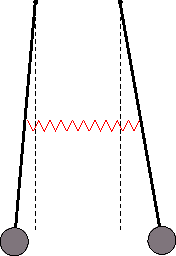
\includegraphics[width=0.6\textwidth]{build/Abb_3.pdf}
        \caption{Abbild der \\gekoppelten Schwingung. \cite{V106}}
        \label{fig:gekoppelt}
      \end{figure}
\end{minipage}
Die Kopplungskonstante
\begin{equation}
    K = \frac{\omega_-^2 -\omega_+^2}{\omega_-^2 + \omega_+^2} = \frac{T_+^2 - T_-^2}{T_+^2 + T_-^2}
    \label{eqn:K}
\end{equation}
der Feder wird als Maß für die Kopplung angesehen.
 % subsection Gekoppelte Schwingungen (end)